\chapter{Aufbau}
\section{Elektrischer Aufbau}




\section{Mechanischer Aufbau}\label{sec:mechanischer_Aufbau}
	\subsection{St�ckliste}
	\begin{enumerate}
		\item Plexiglasrohr
		\item Plexiglasscheibe
		\item 4 M6 Schrauben
		\item 8 M6 Muttern
		\item 8 M6 Unterlagsscheiben
		\item Anschlussteil einen HT-Abwasserrohrs
		\item L�fter
		\item Abstandssensor
		\item Patex 2K Kleber
		\item Sekundenkleber
	\end{enumerate}
	\begin{figure}[htb]
		\centering
		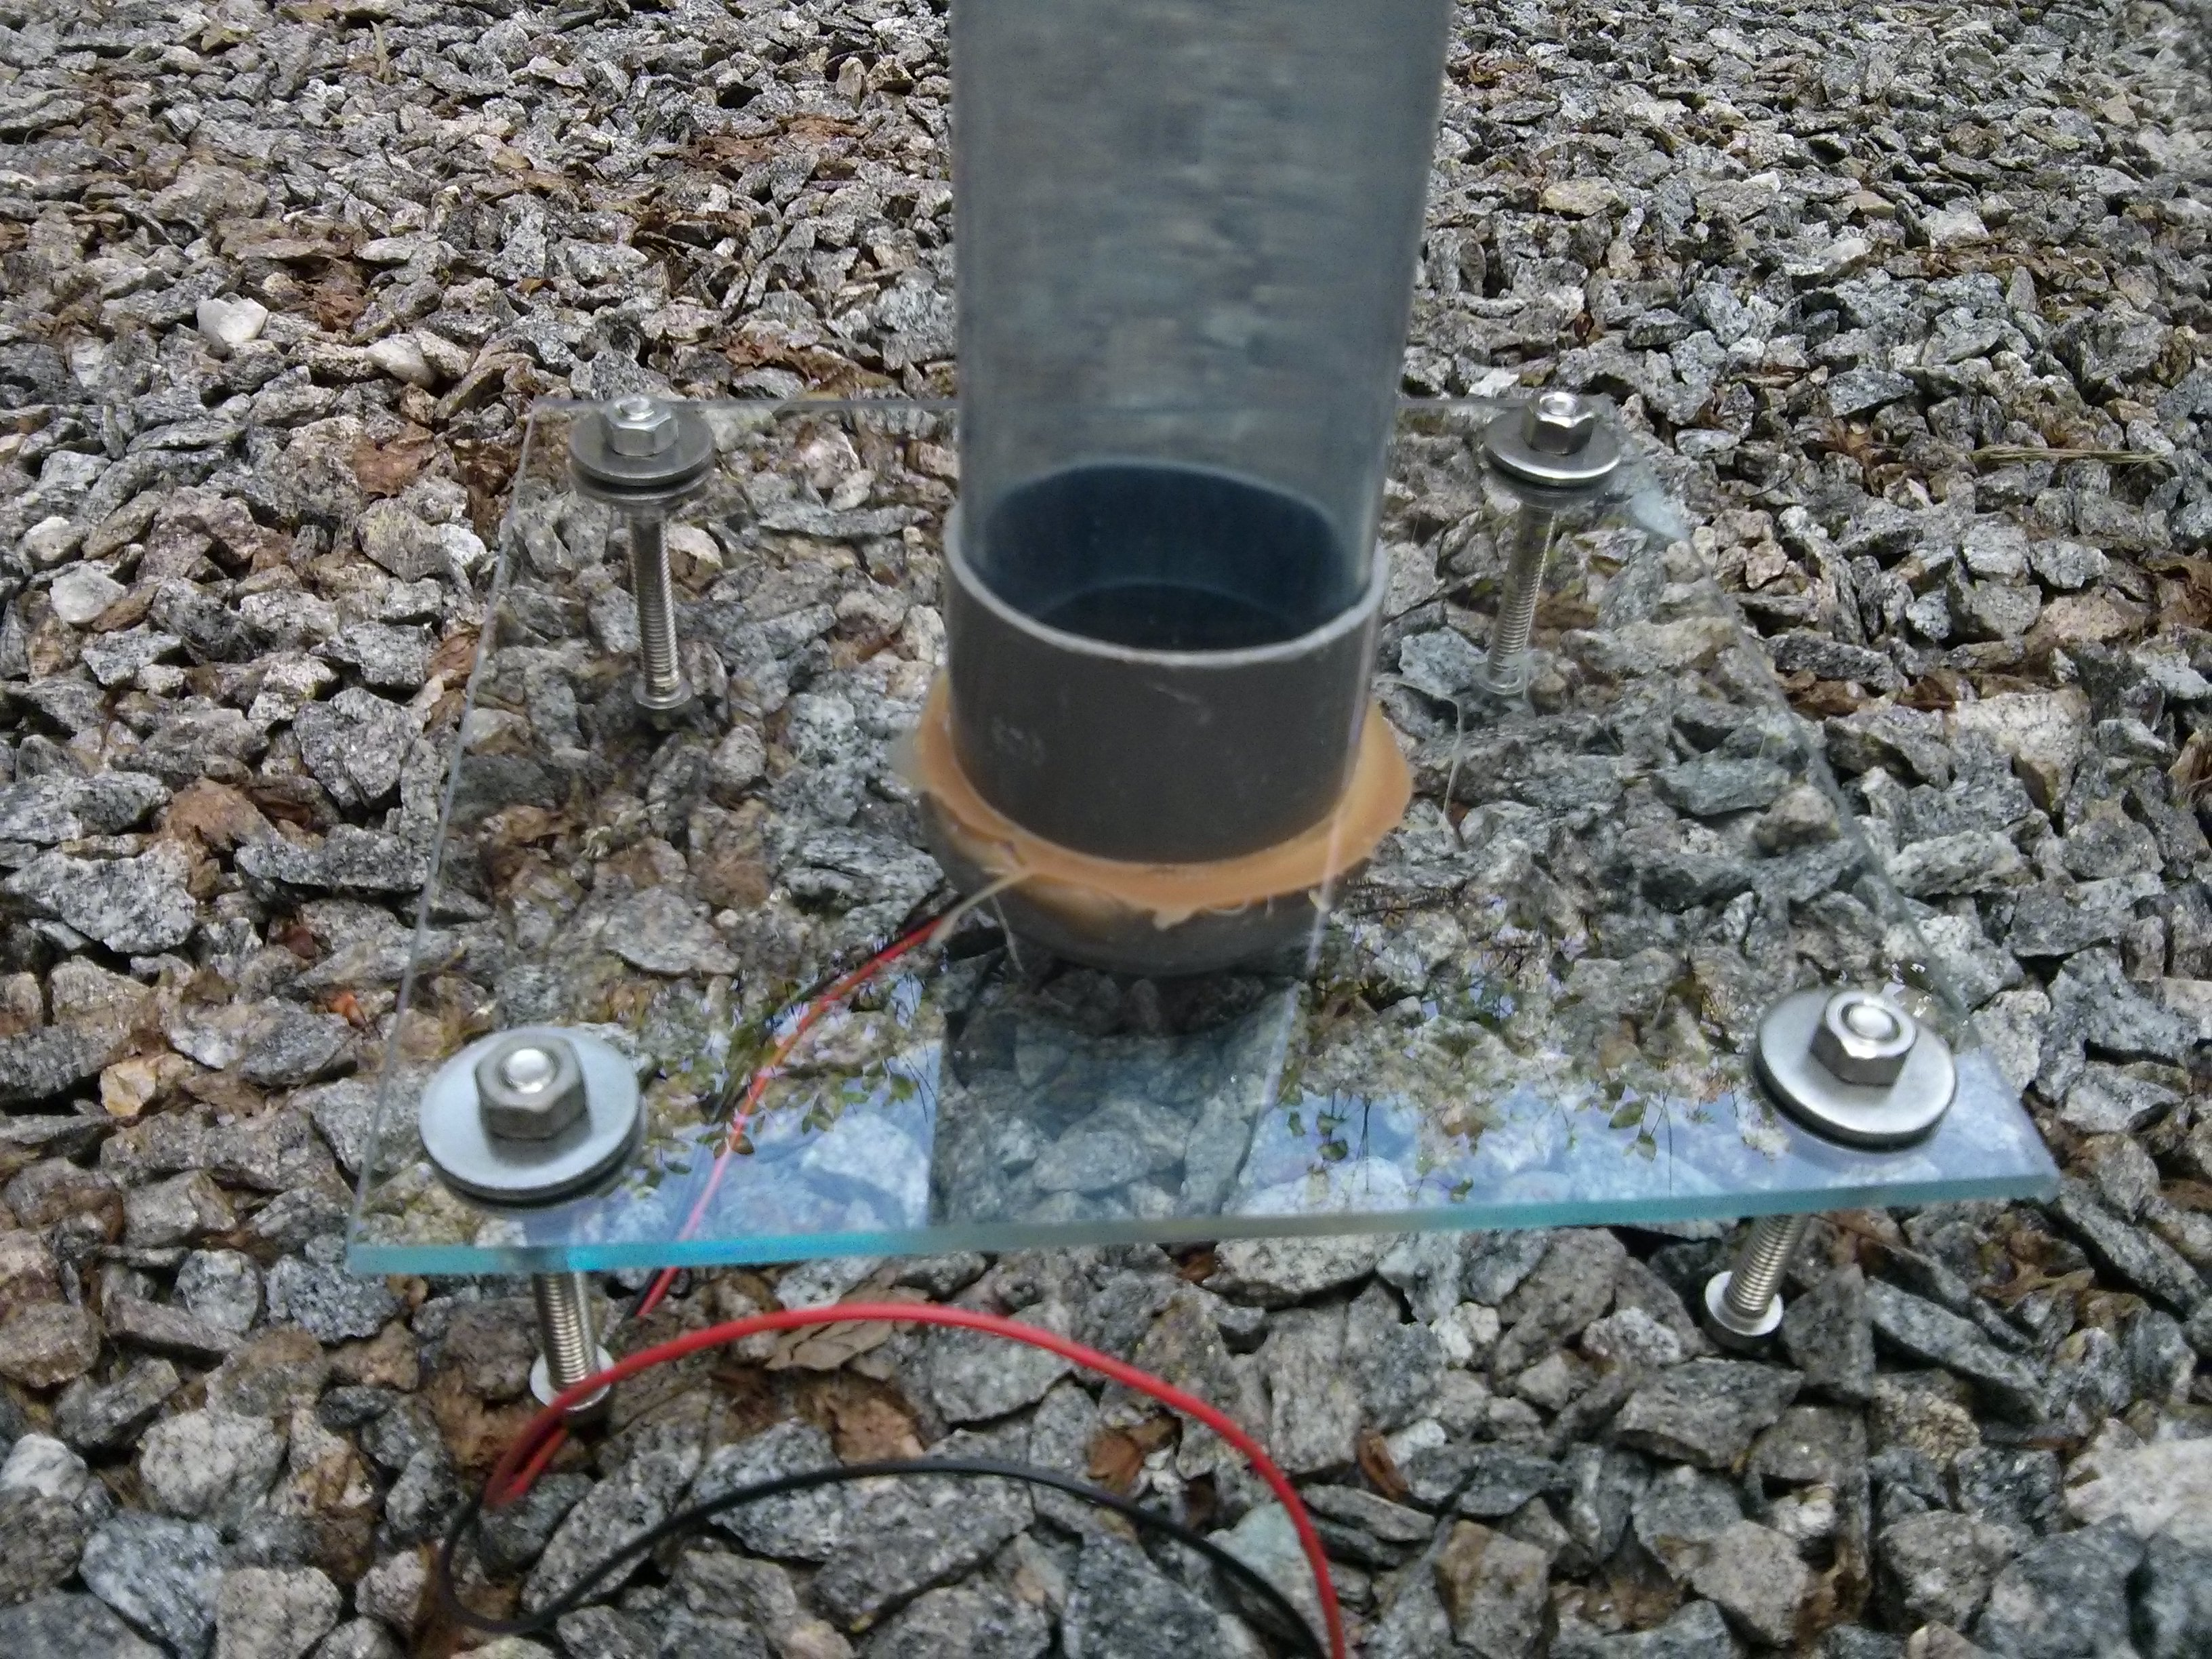
\includegraphics[width=0.8\linewidth]{./Bilder/IMG_20160517_152455}
		\caption{Fertiger mechanischer Aufbau}
		\label{fig:Aufbau_gesamt}
	\end{figure}
\enlargethispage{2em}
\subsection{Beschreibung}
Die Plexiglasscheibe dient als Basis des gesamten mechanischen Aufbaus. In ihrer Mitte befindet sich ein Loch durch welcher das HT-Rohr, bis zur Dichtungsverbreiterungs, genau durchpasst. Obwohl das HT-Rohr schon durch eine Presspassung in der Plexiglasscheibe h�lt wurde es zus�tzlich mit Zweikkomponentenkleber fixiert. In die vier Ecken der Scheibe wurde L�cher gebohrt, durch diese wurden die Schrauben gesteckt und mit den Mutter sowie den Unterlagsscheiben fixiert. Die Schrauben dienen Als F��e f�r den Aufbau. Dies hat fogende Vorteile:
\begin{itemize}
		\item Der L�fter liegt nicht dirkt auf dem Untergrund und kann somit Luft ansaugen.
		\item Der Aufbau steht stabil auf dem Untergrund.
		\item Durch die Verwendung von Schrauben kann ein unebener Untergrund ausgeglichen werden.
\end{itemize}
In die Verbreiterung des HT-Rohrs befindet sich normalerweise eine Gummidichtung. In unserem Fall kann dort aber der L�fter bequem eingeclipst werden. Auf dem L�fter wurde der Abstandssensor mit Sekundenkleber befestigt. Da der Sensor einen Steckanschluss hat und dieser im fertigen Aufbau nicht mehr erreicht werden kann, wurde dieser mit Litzen, am L�fter vorbei unten aus dem HT-Rohr gef�hrt.\\
	\begin{figure}[htb]
			\centering
			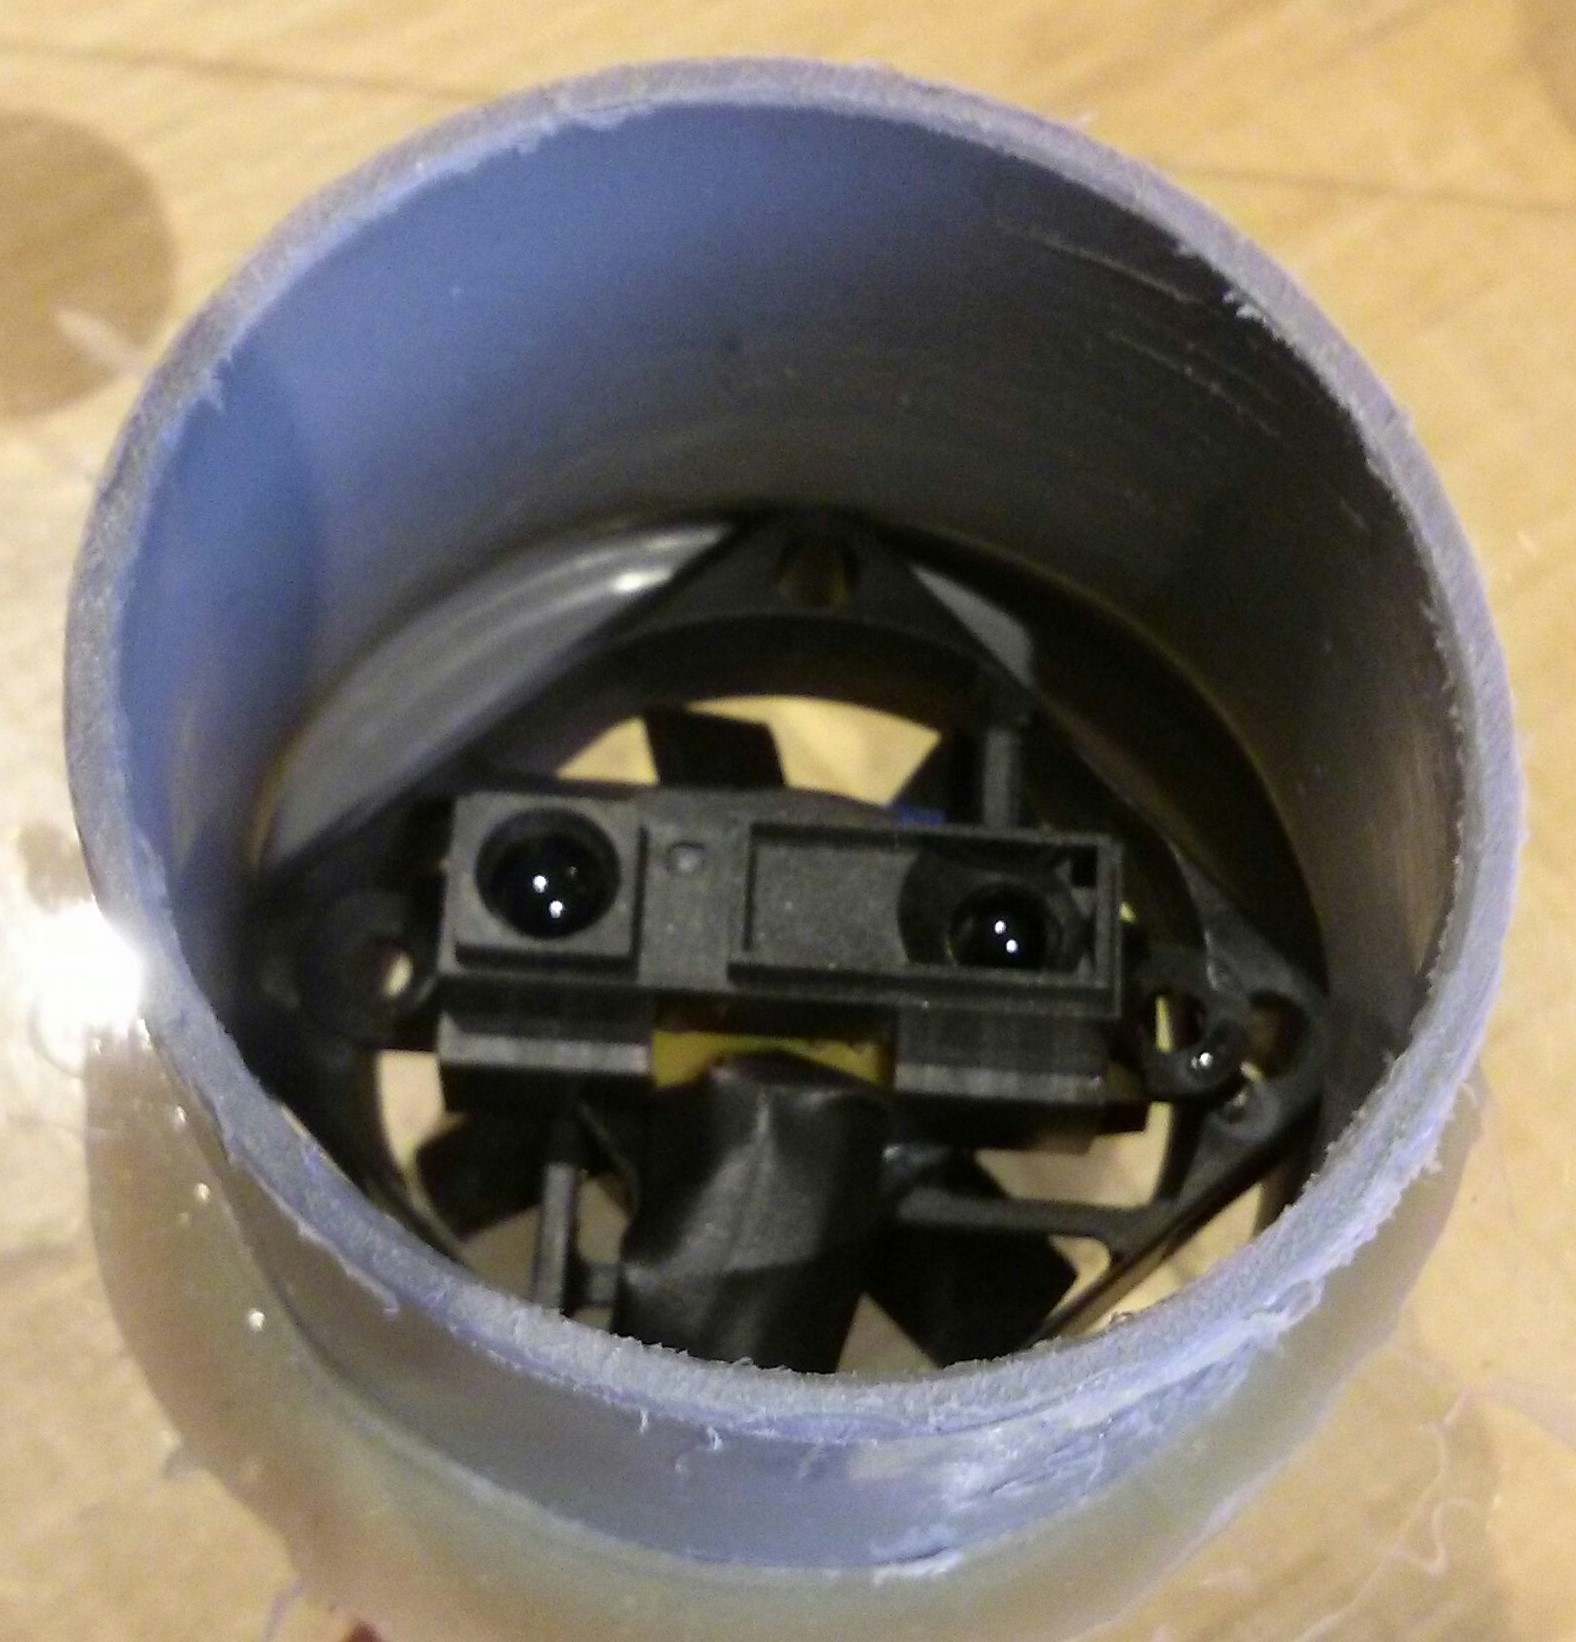
\includegraphics[width=0.7\linewidth]{./Bilder/Luefter_mit_Sensor_im_Rohr}
			\caption{L�fter mit Sensor im HT-Rohr}
			\label{fig:IMG_20160523_191318}
	\end{figure}
In das andere Ende des HT-Rohrs wird das Plexiglas Rohr gesteckt werden, dieses passt ebenfalls genau dort hinein und ist somit durch eine Presspassung fixiert.